\documentclass{beamer}

\usepackage[utf8]{inputenc}
\usepackage{eurosym}
\usepackage{hyperref}
\hypersetup{
    colorlinks = true
    }
\usepackage{graphicx}

%Information to be included in the title page:
\title{GTA Einführung Robotik mit LEGO Mindstorms}
\author{Mattias Schlenker}
\institute{Wilhelm-Ostwald-Gymnasium}
\date{3. Dezember 2020}

\begin{document}

\frame{\titlepage}

\begin{frame}
\frametitle{Achtung, teuer!}
Bitte gebt auf die Roboter acht und widersteht dem Drang, sie umzubauen! Haltet sie von Haustieren und Geschwistern fern!

\begin{itemize}
\item Verlorener EV-Brick? Totalschaden, 400 \EUR 
\item Sensor/Motor verloren/kaputt? 50 \EUR
\item Kleinteile verloren? 1 Stunde LEGO sortieren im Keller!
\end{itemize}
\end{frame}


\begin{frame}
\frametitle{Loslegen mit Makecode}
Ruft die Seite \href{https://makecode.mindstorms.com/}{makecode.mindstorms.com} auf und klickt Euer erstes Programm zusammen: Abwechselnde Gesichtsausdrücke in der Dauerschleife.

\begin{figure}
  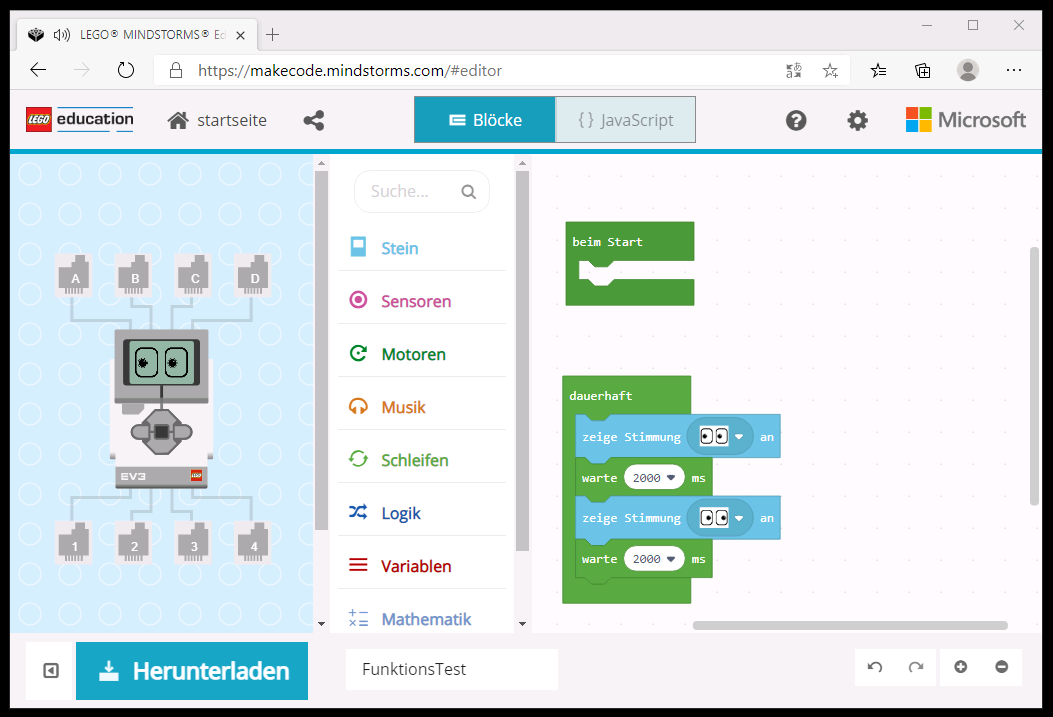
\includegraphics[width=8cm]{mkcd00.png}
  \caption{Makecode Arbeitsfläche}
  \label{fig:mkcd0}
\end{figure}
\end{frame}


\begin{frame}
\frametitle{Herunterladen des Programms}
Gebt dem Programm einen passenden Namen und klickt dann auf ,,Herunterladen'' und schließlich auf ,,Ich habe es  verstanden''

\begin{figure}
  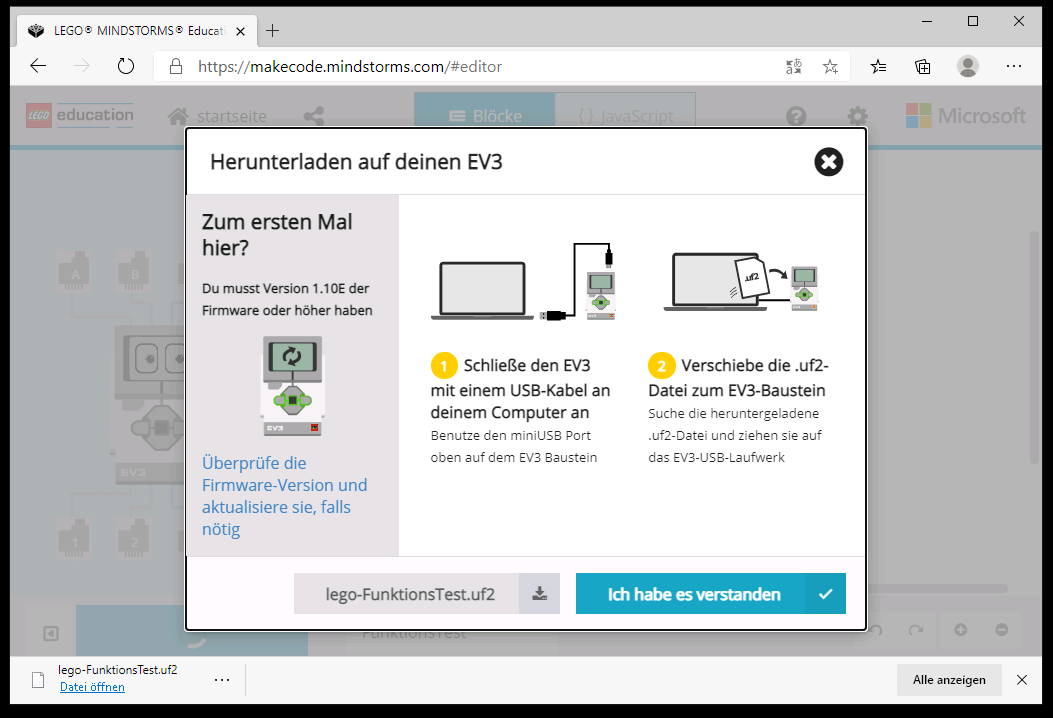
\includegraphics[width=8cm]{mkcd01.png}
  \caption{Makecode Download}
  \label{fig:mkcd1}
\end{figure}
\end{frame}

\begin{frame}
\frametitle{Kopieren des Programms zum Brick}
Verbindet den Roboter mit dem PC und schaltet ihn an. Wartet, bis das Laufwerk ,,EV3'' erscheint. Dann zieht Ihr die UF2-Datei mit dem Programm auf das EV3-Laufwerk:

\begin{figure}
  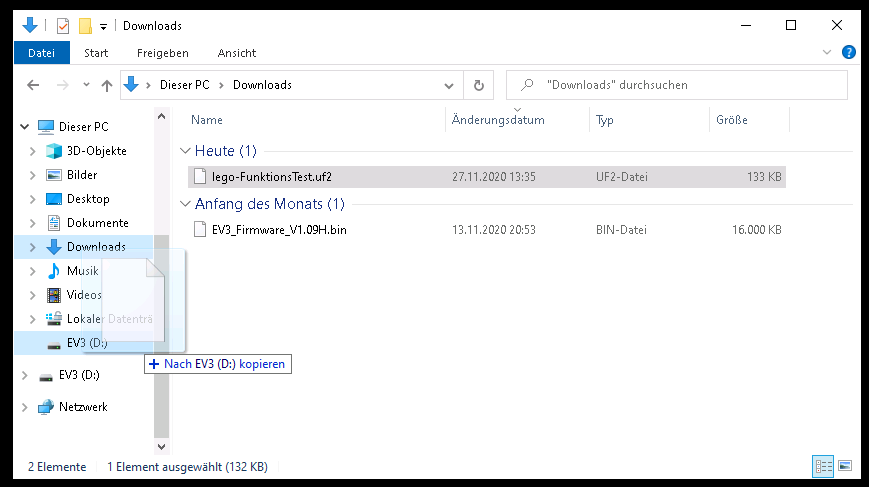
\includegraphics[width=8cm]{mkcd02.png}
  \caption{Dateimanager}
  \label{fig:mkcd2}
\end{figure}
\end{frame}


\begin{frame}
\frametitle{Roboter starten}

Der Roboter sollte nach erfolgreichem Kopieren automatisch neu starten. 

Je nach Einstellung \textbf{startet er gleich} das Programm oder Ihn müsst es \textbf{im Dateimenü des Bricks} suchen. 

\end{frame}

\begin{frame}
\frametitle{Das UF2-Format}

UF2 ist ein hybrides Dateiformat, welches sowohl den \textbf{kompilierten Machinencode (Objektcode)} als auch den menschenlesbaren \textbf{Quellcode enthält}.

\textbf{Bewahrt} Eure UF2-Programme \textbf{gut auf}, denn Ihr könnt diese später weiterbearbeiten! 

Zudem benötigen bei Fragen Herr Brucherseifer und Herr Schlenker Eure Programme. Das geht über die Funktion \textbf{,,teilen''} oder eben durch den \textbf{Versand von UF2-Dateien}.

\end{frame}

\begin{frame}
\frametitle{Weiterbearbeiten eines UF2-Programmes 1}

Geht zur Makecode-Startseite und klickt dort den Button ,,Importieren''. Im erscheinenden Dialog wählt Ihr ,,Datei importieren''.

\begin{figure}
  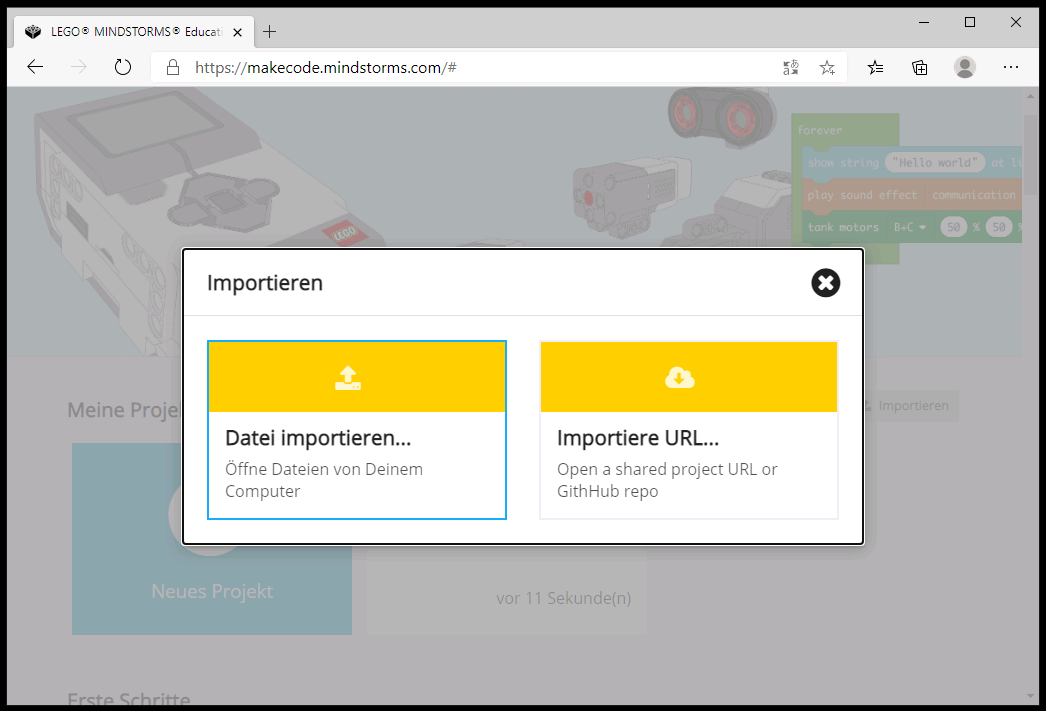
\includegraphics[width=8cm]{mkcd03.png}
  \caption{Importdialog}
  \label{fig:mkcd3}
\end{figure}
\end{frame}

\begin{frame}
\frametitle{Weiterbearbeiten eines UF2-Programmes 2}
Klickt auf ,,Datei auswählen'' und sucht mit dem Dateimanager die zu bearbeitende Datei. Wenn Ihr die richtige Datei ausgewählt ist, klickt Ihr auf ,,Los geht's!''.

\begin{figure}
  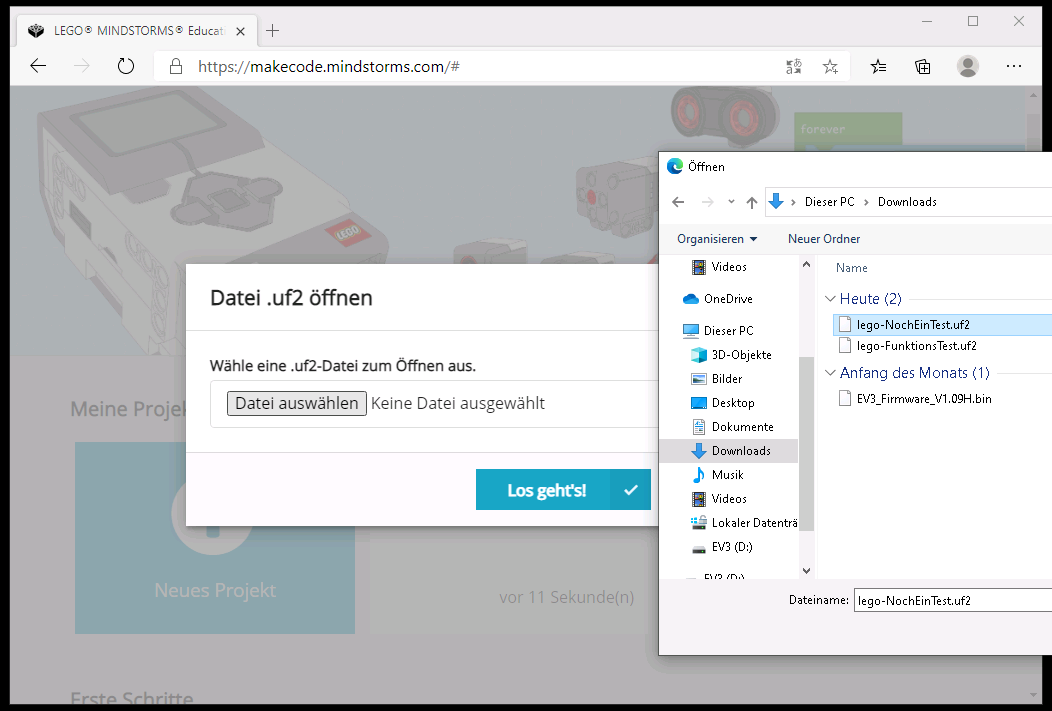
\includegraphics[width=8cm]{mkcd04.png}
  \caption{Importdialog}
  \label{fig:mkcd4}
\end{figure}
\end{frame}

\begin{frame}
\frametitle{Hinweise zum Schluss}
\begin{itemize}
\item
\textbf{Bitte steuert zunächst die Motoren nicht an!} Ihr dürft gerne \textbf{Sensoren oder Knopfdrücke auslesen} und mit \textbf{Tönen oder Anzeigen auf dem Display}  quittieren.
\item Wenn Ihr sicherer seid, fangt mit \textbf{einfachen Programmen} an: Mit \textbf{50\% Motordrehzahl} anfahren und sofort stoppen, wenn ein Hindernis erkannt wird...
\item \textbf{Hausaufgabe: Wieviele Grad muss jedes Rad} (jeweils in Gegenrichtung) \textbf{drehen}, damit der Roboter genau gegen Fahrtrichtung steht? Tipp: Rechnet in der Einheit ,,LEGO-Noppen\footnote{Zur Kontrolle: Das Rastermaß von Lego sind ca. 7,9mm. Ein Lego-Baustein mit 4 × 2 Noppen entspricht im Maßstab 1:7 einem normalen Backstein mit 9 × 4½ × 3 Zoll.}'': Die Kreiszahl Pi und die Maßeinheit kürzt sich heraus und am Ende steht ein schöner Bruch. Die beste Lösung bekommt einen Schoko- oder Limopreis!
\end{itemize}
\end{frame}

% \begin{frame}
% \frametitle{Der Anspruch – der Schule und von uns selbst}
% \begin{itemize}
% \item  Wir lernen die Interaktion von Elektronik und physischer Welt
% \item  Unsere Arbeit ist eher ingenieurstechnisch als wissenschaftlich
% \item Physik und Technik: hier eher qualitativ als quantitativ
% \item  Wir machen Fehler und lernen daraus!
% \item Wir lernen auch aus Fehlern anderer – hilft schneller zu sein
% \item  Wir arbeiten gemeinsam auf Wettbewerbe hin
% \item  Jeder lernt alles: Programmieren und Konstruktion 
% \item  Bei Ad-Hoc-Wettbewerben dennoch Rollen im Team – Konstrukteur:innen, Programmierer:innen und Integrator:innen 
% \end{itemize}
% \end{frame}

% \begin{frame}
% \frametitle{Die Werkzeuge – und Umgang damit}
% \begin{itemize}
% \item  LEGO Technik zur Konstruktion
% \item  Mindstorm liefern autonome Steuereinheit, Sensoren, Aktoren
% \item Programmierung in \href{https://makecode.mindstorms.com/}{Makecode} (,,Klötzchen''), Python (Fortgeschrittene)
% \item  Wir lernen Dokumentation von Soft- und Hardware
% \item  Wir arbeiten strukturiert mit Versionierung \& Kommentierung!
% \item Wir benutzen ,,Rubber-Ducking'' zur Fehlersuche
% \item  Am Ende: Stand festhalten, Code sichern, Arbeitsplatz aufräumen!
% \item Materialien: Austausch LernSax, Folien und Beispielcode auf \href{https://github.com/mschlenker/GtaRoboter2020}{GitHub}
% \end{itemize}
% \end{frame}




\end{document}
